
\chapter{Principe de filtre dérivateur}

Il existe de nombreux types de traitement d'images. Celui que l'on utilisera ici est un filtre dérivateur.
Dans ce cas, on peut approcher la dérivée par une différence finie tel que :
\begin{equation}
\frac{\partial f}{\partial x} \simeq f (x+1) - f(x)
\end{equation}
On écrit aussi :

\begin{equation}
\frac{\partial f}{\partial x} \simeq g_{-1} f(x+1) + g_0 f(x)
\end{equation}
Soit :

\begin{equation}
\frac{\partial f}{\partial x} \simeq \sum_{k=-1}^{k=0} g_k f(x-k)
\end{equation}
Ce qui correspond à une opération de convolution et donc de filtrage numérique.

\bigskip

Cependant ceci est vrai pour un cas en une dimension. Il faut donc généraliser au cas en 2D pour le traitement de l'image.
En général, on nous donne la formule de calcul suivante pour le filtrage linéaire d'une image f de taille M x N avec un masque de taille m x n.
\begin{equation}
g(x,y) = \sum_{s=-a}^a \sum_{t=-b}^b w(s,t)f(x+s,y+t)
\end{equation}
où \textit{a}=(\textit{m}-1)/2 et \textit{b}=(\textit{n}-1)/2.

\bigskip

Cette équation doit-être appliquée pour tout les points de l'image afin d'obtenir une image filtrée. Étant donné que notre masque de filtrage se base sur les pixels autour de celui \og{}selectionné\fg{}, il conviendra d'éviter les effets de bords. On choisira d'ajouter des zéros autour de l'image.

\chapter{Développement}

\section{Conversion de l'image en niveaux de gris}
Le filtrage s'effectue sur une image simple canal (une seule composante entre 0 et 255, le gris). En revanche le RGB (Red Green Blue) fourni par la caméra utilise 3 canaux. Le conversion s'effectue comme suit :
\begin{equation}
Y = 0.299R + 0.587G + 0.114B
\end{equation}

\section{Implémentation du filtrage dérivateur}
On utilisera 2 masques de dérivation différents.
\begin{itemize}
	\item Masque de Sobel \\ \begin{equation}
			G_x=\begin{bmatrix}
					-1 & 0 & 1 \\
					-2 & 0 & 2 \\
					-1 & 0 & 1
				\end{bmatrix}
			G_y=\begin{bmatrix}
					1 & 2 & 1 \\
					0 & 0 & 0 \\
					-1 & -2 & -1
				\end{bmatrix}
		  \end{equation} 
    \item Masque de Prewitt \\ \begin{equation}
			G_x=\begin{bmatrix}
					-1 & 0 & 1 \\
					-1 & 0 & 1 \\
					-1 & 0 & 1
				\end{bmatrix}
			G_y=\begin{bmatrix}
					1 & 1 & 1 \\
					0 & 0 & 0 \\
					-1 & -1 & -1
				\end{bmatrix}
		  \end{equation} 
\end{itemize}
Pour chaque masque l'image dérivée de sortie sera la norme du gradient en chaque pixel c'est à dire :
\begin{equation}
|G| = \sqrt{G_x^2 + G_y^2}
\end{equation}

\section{Questions et Code C++}
Nous allons donc développer nos filtres en C++ en complétant les fichiers fournis. Il sera utilisé une structure \lstinline{MAPS::IplImage} contenant la plupart des informations d'une image. Le plus important est un tableau contenant les informations de chaque pixel.\\
En niveau de gris, le tableau associé à un pixel est un \lstinline{unsigned char} codant le niveau. En RGB, le tableau se visualise par groupe de 3 cases. Ces trois cases contiennent chacune un \lstinline{unsigned char} correspondant aux niveaux de rouge, vert et bleu de chaque pixel.

\subsection{Question 1}
On donne le pseudo-code capable d'appliquer une fonction F à chaque pixel d'une image en niveau de gris. On utilise \lstinline{img} qui correspond à l'adresse du premier pixel dans le tableau.
\noindent\fbox{%
\begin{minipage}{\dimexpr\linewidth-2\fboxsep-2\fboxrule\relax}
\begin{algorithmic}
\State $i\gets 0$
\For{($i$=0 ; $i$ < taille($img$); $i$++)}
  \Call{F}{$img$[$i$]}
\EndFor
\end{algorithmic}
\end{minipage}% 
}

\subsection{Question 2}
De même que pour la question 1, sauf qu'ici on veut appliquer la fonction à une image couleur RGB.\\
\noindent\fbox{%
\begin{minipage}{\dimexpr\linewidth-2\fboxsep-2\fboxrule\relax}
\begin{algorithmic}
\State $i\gets 0$
\For{($i$=0 ; $i$ < taille($img$); $i$++)}
  \Call{F}{$img$[3*$i$],$img$[3*$i$+1],$img$[3*$i$+2]}
\EndFor
\end{algorithmic}
\end{minipage}% 
}

\subsection{Question 3}
Dans la structure \lstinline{MAPS::IplImage} les pixels sont stockés dans un tableau ligne après ligne. C'est à dire que la première ligne de pixels de l'image occupe les premières cases du tableau, puis la seconde ligne occupe les cases suivantes, etc...
Dans une image couleur RGB, on se souvient aussi que chaque pixel prend 3 cases dans le tableau.
Donc pour accèder au pixel d'indice (i,j), on fait :
\noindent\fbox{%
\begin{minipage}{\dimexpr\linewidth-2\fboxsep-2\fboxrule\relax}
\begin{algorithmic}
\State $pixel\gets (j*largeur*3)+(3*i$)
\end{algorithmic}
\end{minipage}% 
}
où \lstinline{largeur} correspond à la largeur de l'image (en nombre de pixels).

\subsection{Question 4}
Lors de la conversion RGB vers niveau de gris, il faut s'assurer que le niveau de gris ne soit pas supérieur à 255 puisque sur 8 bits on peut stocker des valeurs décimales allant de 0 à 255.\\
En réalité ce n'est pas un vrai problème. En effet on remarque que dans notre formule de calcul du niveau de gris, la somme des coefficients multipliant chaque canal est égale à 1 (0.299+0.587+0.114=1). Cela signifie que quelque soit la valeur de notre pixel couleur (de (0,0,0) à (255,255,255)), le résulat sera toujours compris entre 0 et 255.

\subsection{Code C++}
\subsubsection{RGB to Gray}
On se propose maintenant de coder réellement notre filtre. On commence par notre fonction de conversion :
\cpp
\begin{lstlisting}
void SobelComponent::rgb2gray(IplImage const& src, IplImage& dst)
{
	int i;
	for(i=0;i<src.width*src.height;i++)
	{
		dst.imageData[i]=src.imageData[3*i]*0.299+src.imageData[3*i+1]*0.587+src.imageData[3*i+2]*0.114;
	}
	
}
\end{lstlisting}
Cette fonction est relativement simple. Elle se contente d'implémenter la formule de conversion donnée, en prenant garde de parcourir correctement (sans erreur d'indice) le tableau image en RGB. Pour cela il suffit de bien se souvenir qu'un pixel occupe 3 cases. Il faut également faire attention à l'ordre des composantes (rouge, puis vert et enfin bleu).

\subsubsection{Convolution}
On passe ensuite à la fonction réalisant la convolution entre notre masque et notre image. Celle-ci prend en entrée les coordonnées x et y correspondant au point à traiter, ainsi qu'un masque. Ceci nous permet d'utiliser la même fonction convolution quelque soit le masque utilisé (ici Sobel ou Prewitt) puisqu'il est passé en paramètre.
\cpp
\begin{lstlisting}
int SobelComponent::convolution(IplImage const& src, int x, int y, int const* mask)
{ 
	int R=0;
	// On parcourt les pixels autour du pixel (x,y)
	for(int i=-1;i<=1;i++) // Parcours en hauteur
	{
		for(int j=-1;j<=1;j++) // Parcours en largeur
			R+=mask[3*(i+1)+(j+1)]*src.imageData[(src.width*(i+x))+(j+y)]; // Application du masque
	}
	return R;	// On retourne la nouvelle valeur du pixel (x,y)
}
\end{lstlisting}
C'est encore une fois une application de la formule donnée. Nos 2 boucles \lstinline{for} correspondent à l'imbrication des 2 sommes.

\subsubsection{Sobel}
On programme maintenant la fonction qui effectue le calcul complet de l'image en utilisant le masque de Sobel. On rappelle que l'image de sortie correspond à :
\begin{equation}
|G| = \sqrt{G_x^2 + G_y^2}
\end{equation}
Notre fonction se contentera donc d'appliquer le produit de convolution entre les points et chacun des 2 matrices. On applique ensuite la formule ci-dessus et on n'oublie pas de normaliser notre pixel.
\cpp
\begin{lstlisting}
void SobelComponent::compute_sobel(IplImage const& src, IplImage& dst)
{  
	//Masque de SOBEL
	int Gx[9] ={-1,0,1,-2,0,2,-1,0,1};
	int Gy[9] ={1,2,1,0,0,0,-1,-2,-1};
	int x,y;

	for(int i=1;i<src.height-1;i++) // De 1 à la hauteur-1 pour éviter l'effet de bord
	{
		for(int j=1;j<src.width-1;j++) // De 1 à la largeur-1 pour éviter l'effet de bord
		{
		// On applique le masque de Sobel au pixel (i,j)
		x=convolution(src,i,j,Gx);
		y=convolution(src,i,j,Gy);
		int g=sqrt((double)(x*x)+(y*y));
		g=max(min(g,255),0); // On vérifie que la valeur de sortie est entre 0 et 255
		dst.imageData[i*dst.width+j]=g; // On écrit dans l'image de sortie
		}
	}
}
\end{lstlisting}

\subsubsection{Prewitt}
De même on programme une fonction pour le masque de Prewitt. Son fonctionnement est strictement identique à la fonction précédente. Seul le masque change.
\cpp
\begin{lstlisting}
void SobelComponent::compute_per(IplImage const& src, IplImage& dst){ 
	//Masque de Prewitt
	int Gx[9] ={-1,0,1,-1,0,1,-1,0,1};
	int Gy[9] ={1,1,1,0,0,0,-1,-1,-1};
	int x,y;
	for(int i=1;i<src.height-1;i++){
		for(int j=1;j<src.width-1;j++){
			x=convolution(src,i,j,Gx);
			y=convolution(src,i,j,Gy);
			int g=sqrt((double)(x*x)+(y*y));
			g=max(min(g,255),0);
			dst.imageData[i*dst.width+j]=g;
		}
	}
}
\end{lstlisting}

\subsection{Question 5}
Après avoir créé notre module RTMaps on effectue nos tests. On obtient les images ci-dessous. On peut voir une main venir de la gauche de l'image, tenant un stylo.
\begin{figure}[!h]
   \centering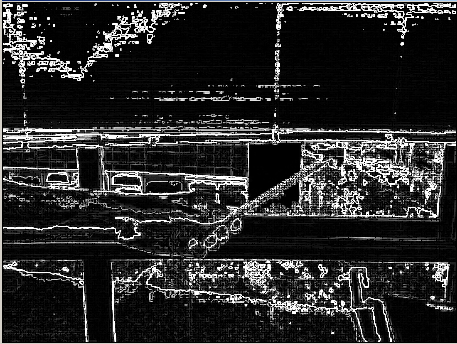
\includegraphics[width=0.7\textwidth]{pictures/sobel_comp.png}
   \caption{Masque de Sobel}
\end{figure}
\begin{figure}[!h]
   \centering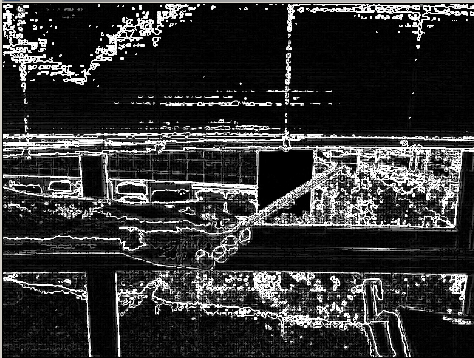
\includegraphics[width=0.7\textwidth]{pictures/prewitt_comp.png}
   \caption{Masque de Prewitt}
\end{figure}

L'image de sortie avec le masque de Prewitt semble contenir plus de points clairs. On a donc une certaine impression de \og bruit\fg{} dans les zones où il y a de nombreuses lignes (par exemple au niveau des visages).
L'image avec le masque de Sobel semble être moins \og bruitée\fg{} et les contours semblent plus nets.

\subsection{Question 6}
Les autres types de masques dérivateurs utilisés sont, entre autres, les masques de Roberts, de Kirsch ou de Robinson.